\documentclass{beamer}
\usepackage{color,amsmath}
\usepackage{subfigure}
\usepackage{booktabs}
\usepackage{framed}
\usepackage{comment}

\def\vf{\vfill}

%%%%%%%%%%%%%%%%%%%%%%%%%%
\title[]{Soc 596: Computational Social Science}
\author[]{Matthew J. Salganik\\Department of Sociology\\Princeton University}
\date[]{01-01-Introduction to computational social science
\vfill
\begin{flushright}
\vspace{0.6in}

\includegraphics[width=0.1\textwidth]{figures/cc.png}
\end{flushright}
}
\begin{document}
%%%%%%%%%%%%%%%%%%%%%%%%%%
\frame{\titlepage}
%%%%%%%%%%%%%%%%%%%%%%%%%%
\begin{frame}

\begin{center}
\LARGE{What is computational social science?}
\end{center}

\end{frame}
%%%%%%%%%%%%%%%%%%%%%%%%%%%
\begin{frame}

\begin{center}
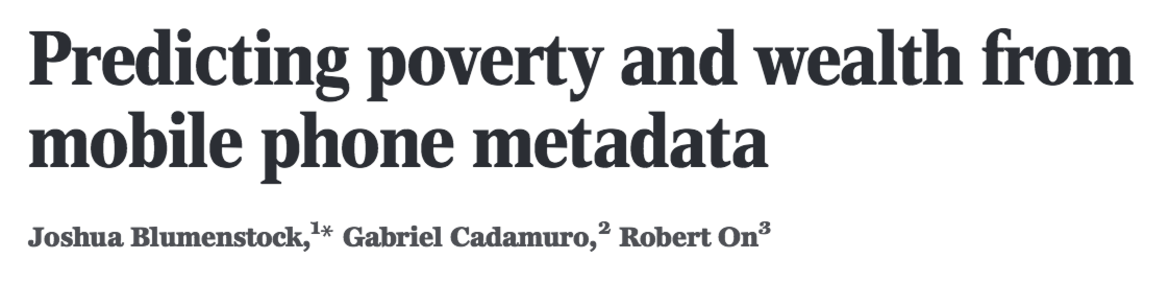
\includegraphics[width=0.9\textwidth]{figures/blumenstock_predicting_2015}
\end{center}

\vf
\TINY{\textcolor{blue}{\url{http://dx.doi.org/10.1126/science.aac4420}}}

\end{frame}
%%%%%%%%%%%%%%%%%%%%%%%%%%%
\begin{frame}

\begin{center}
\only<1>{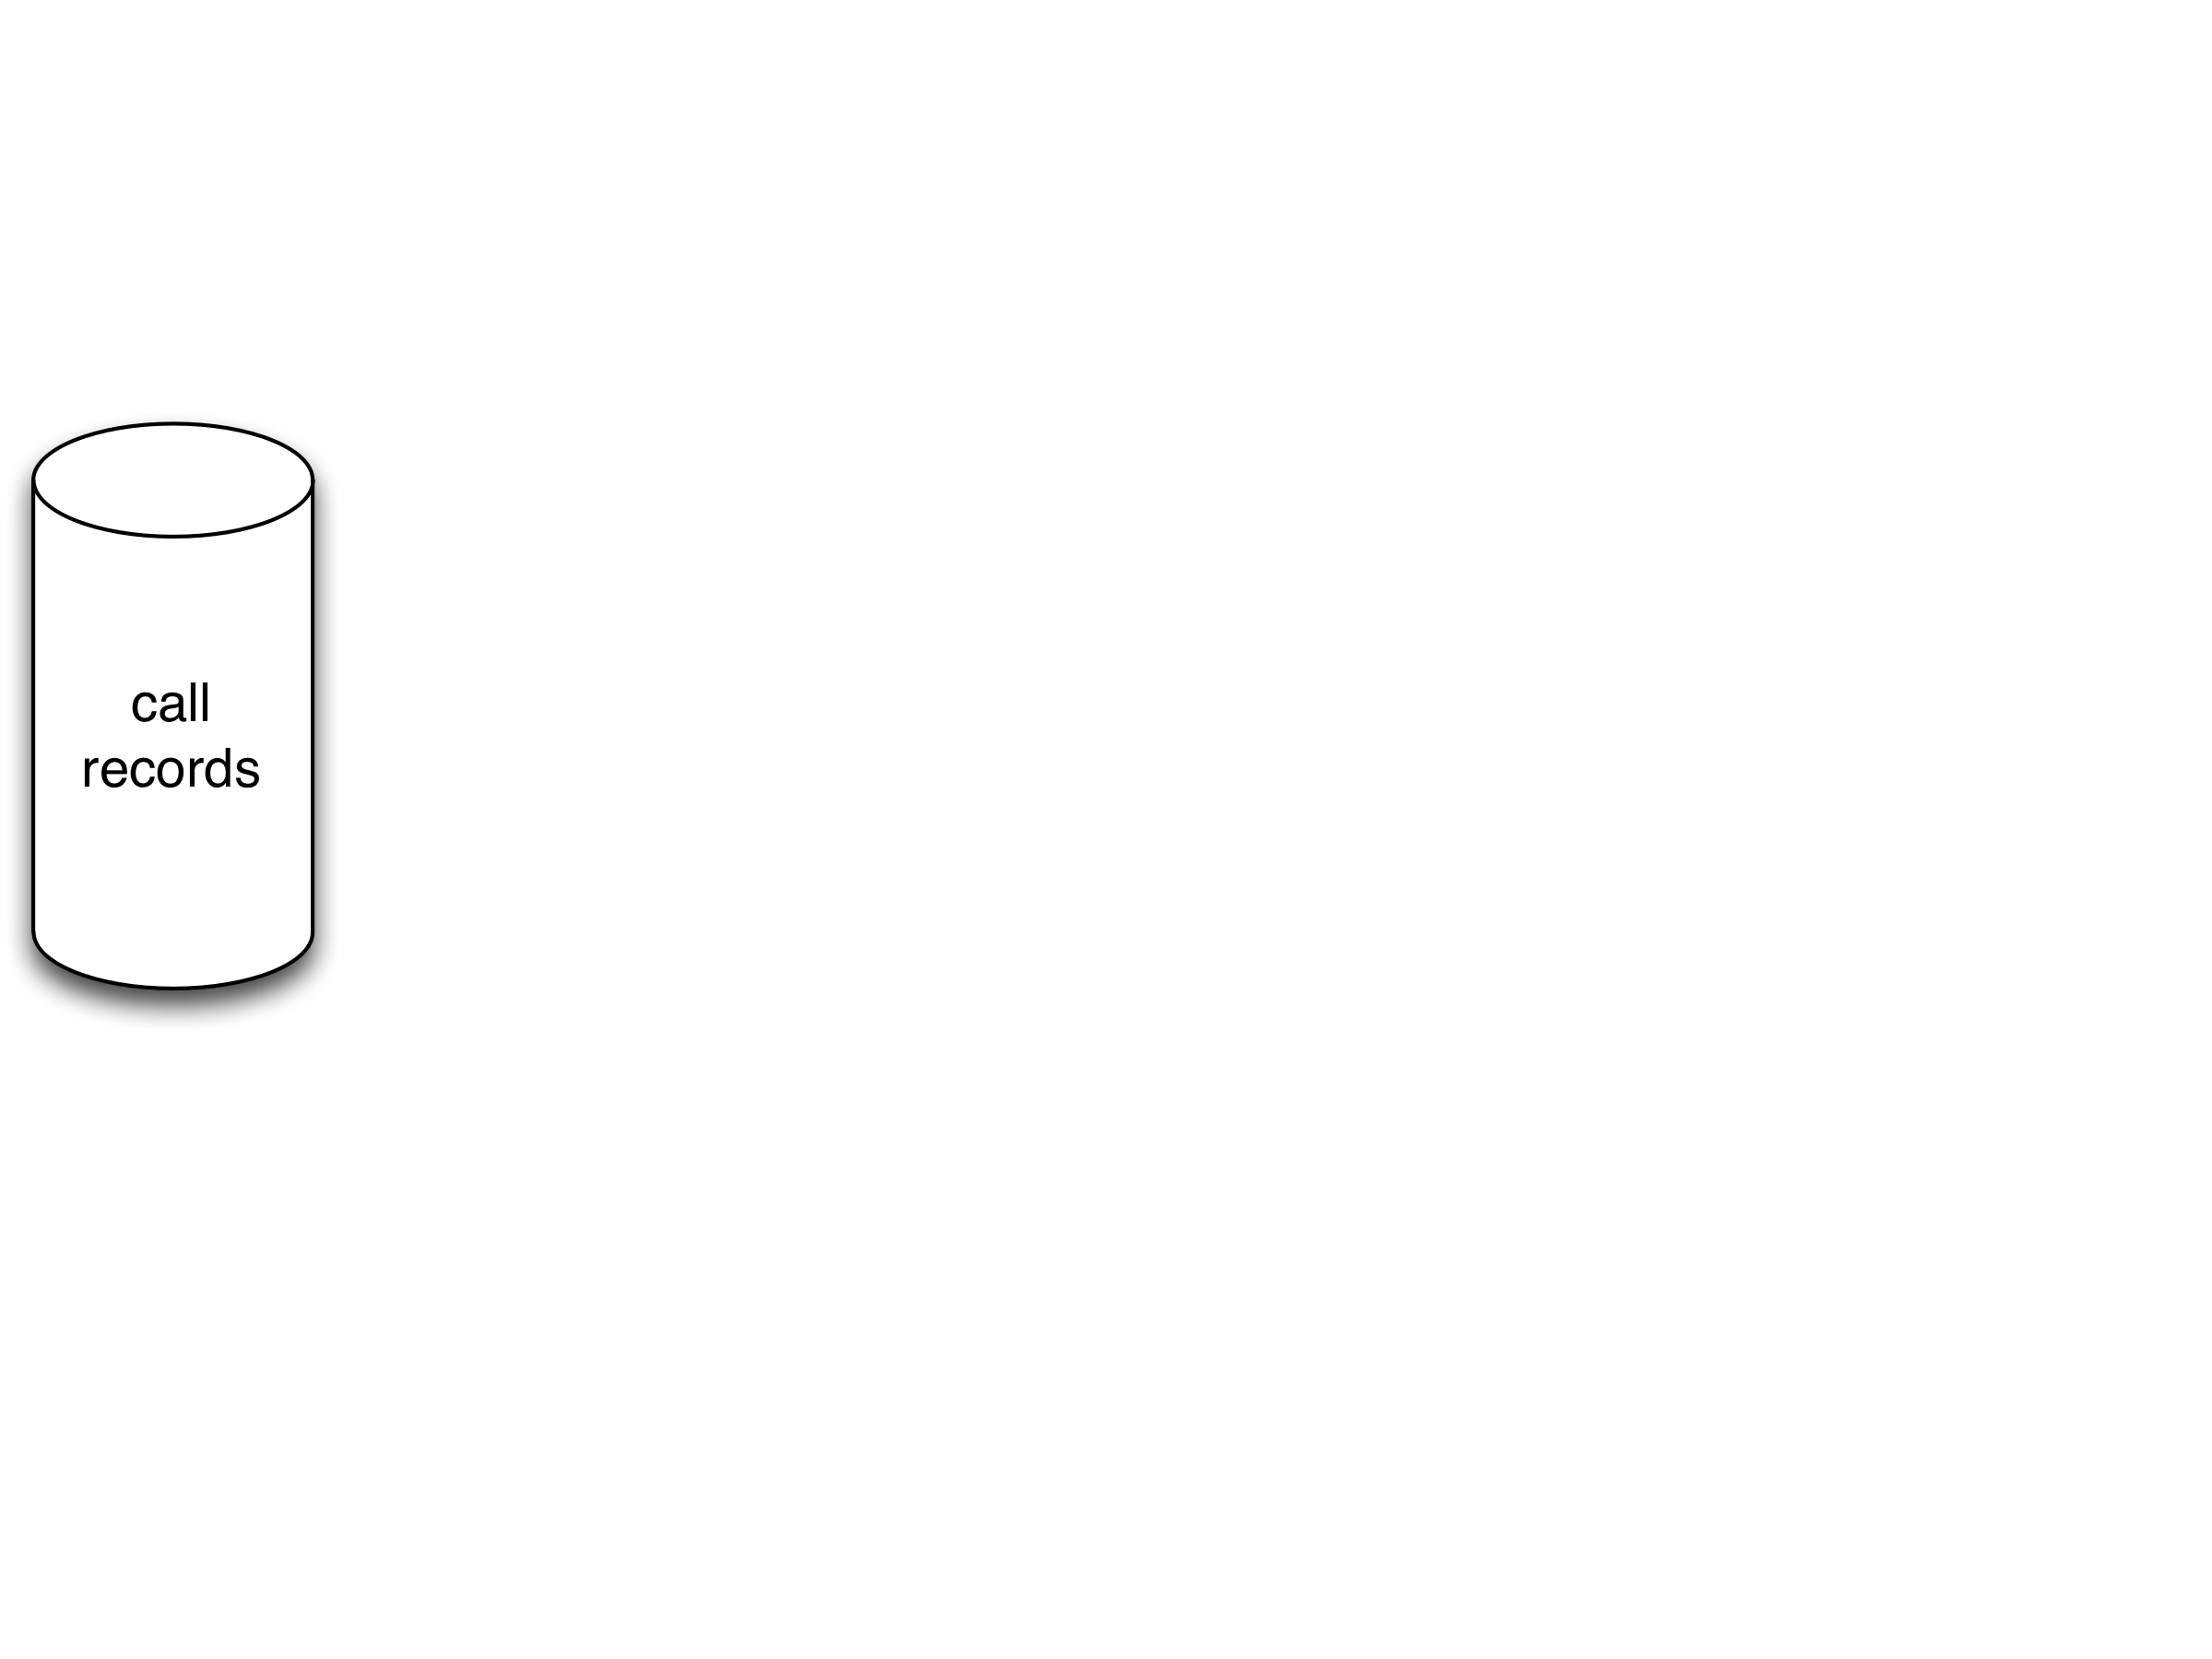
\includegraphics[width=0.9\textwidth]{figures/blumenstock_predicting_2015_schematic_1}}
\only<2>{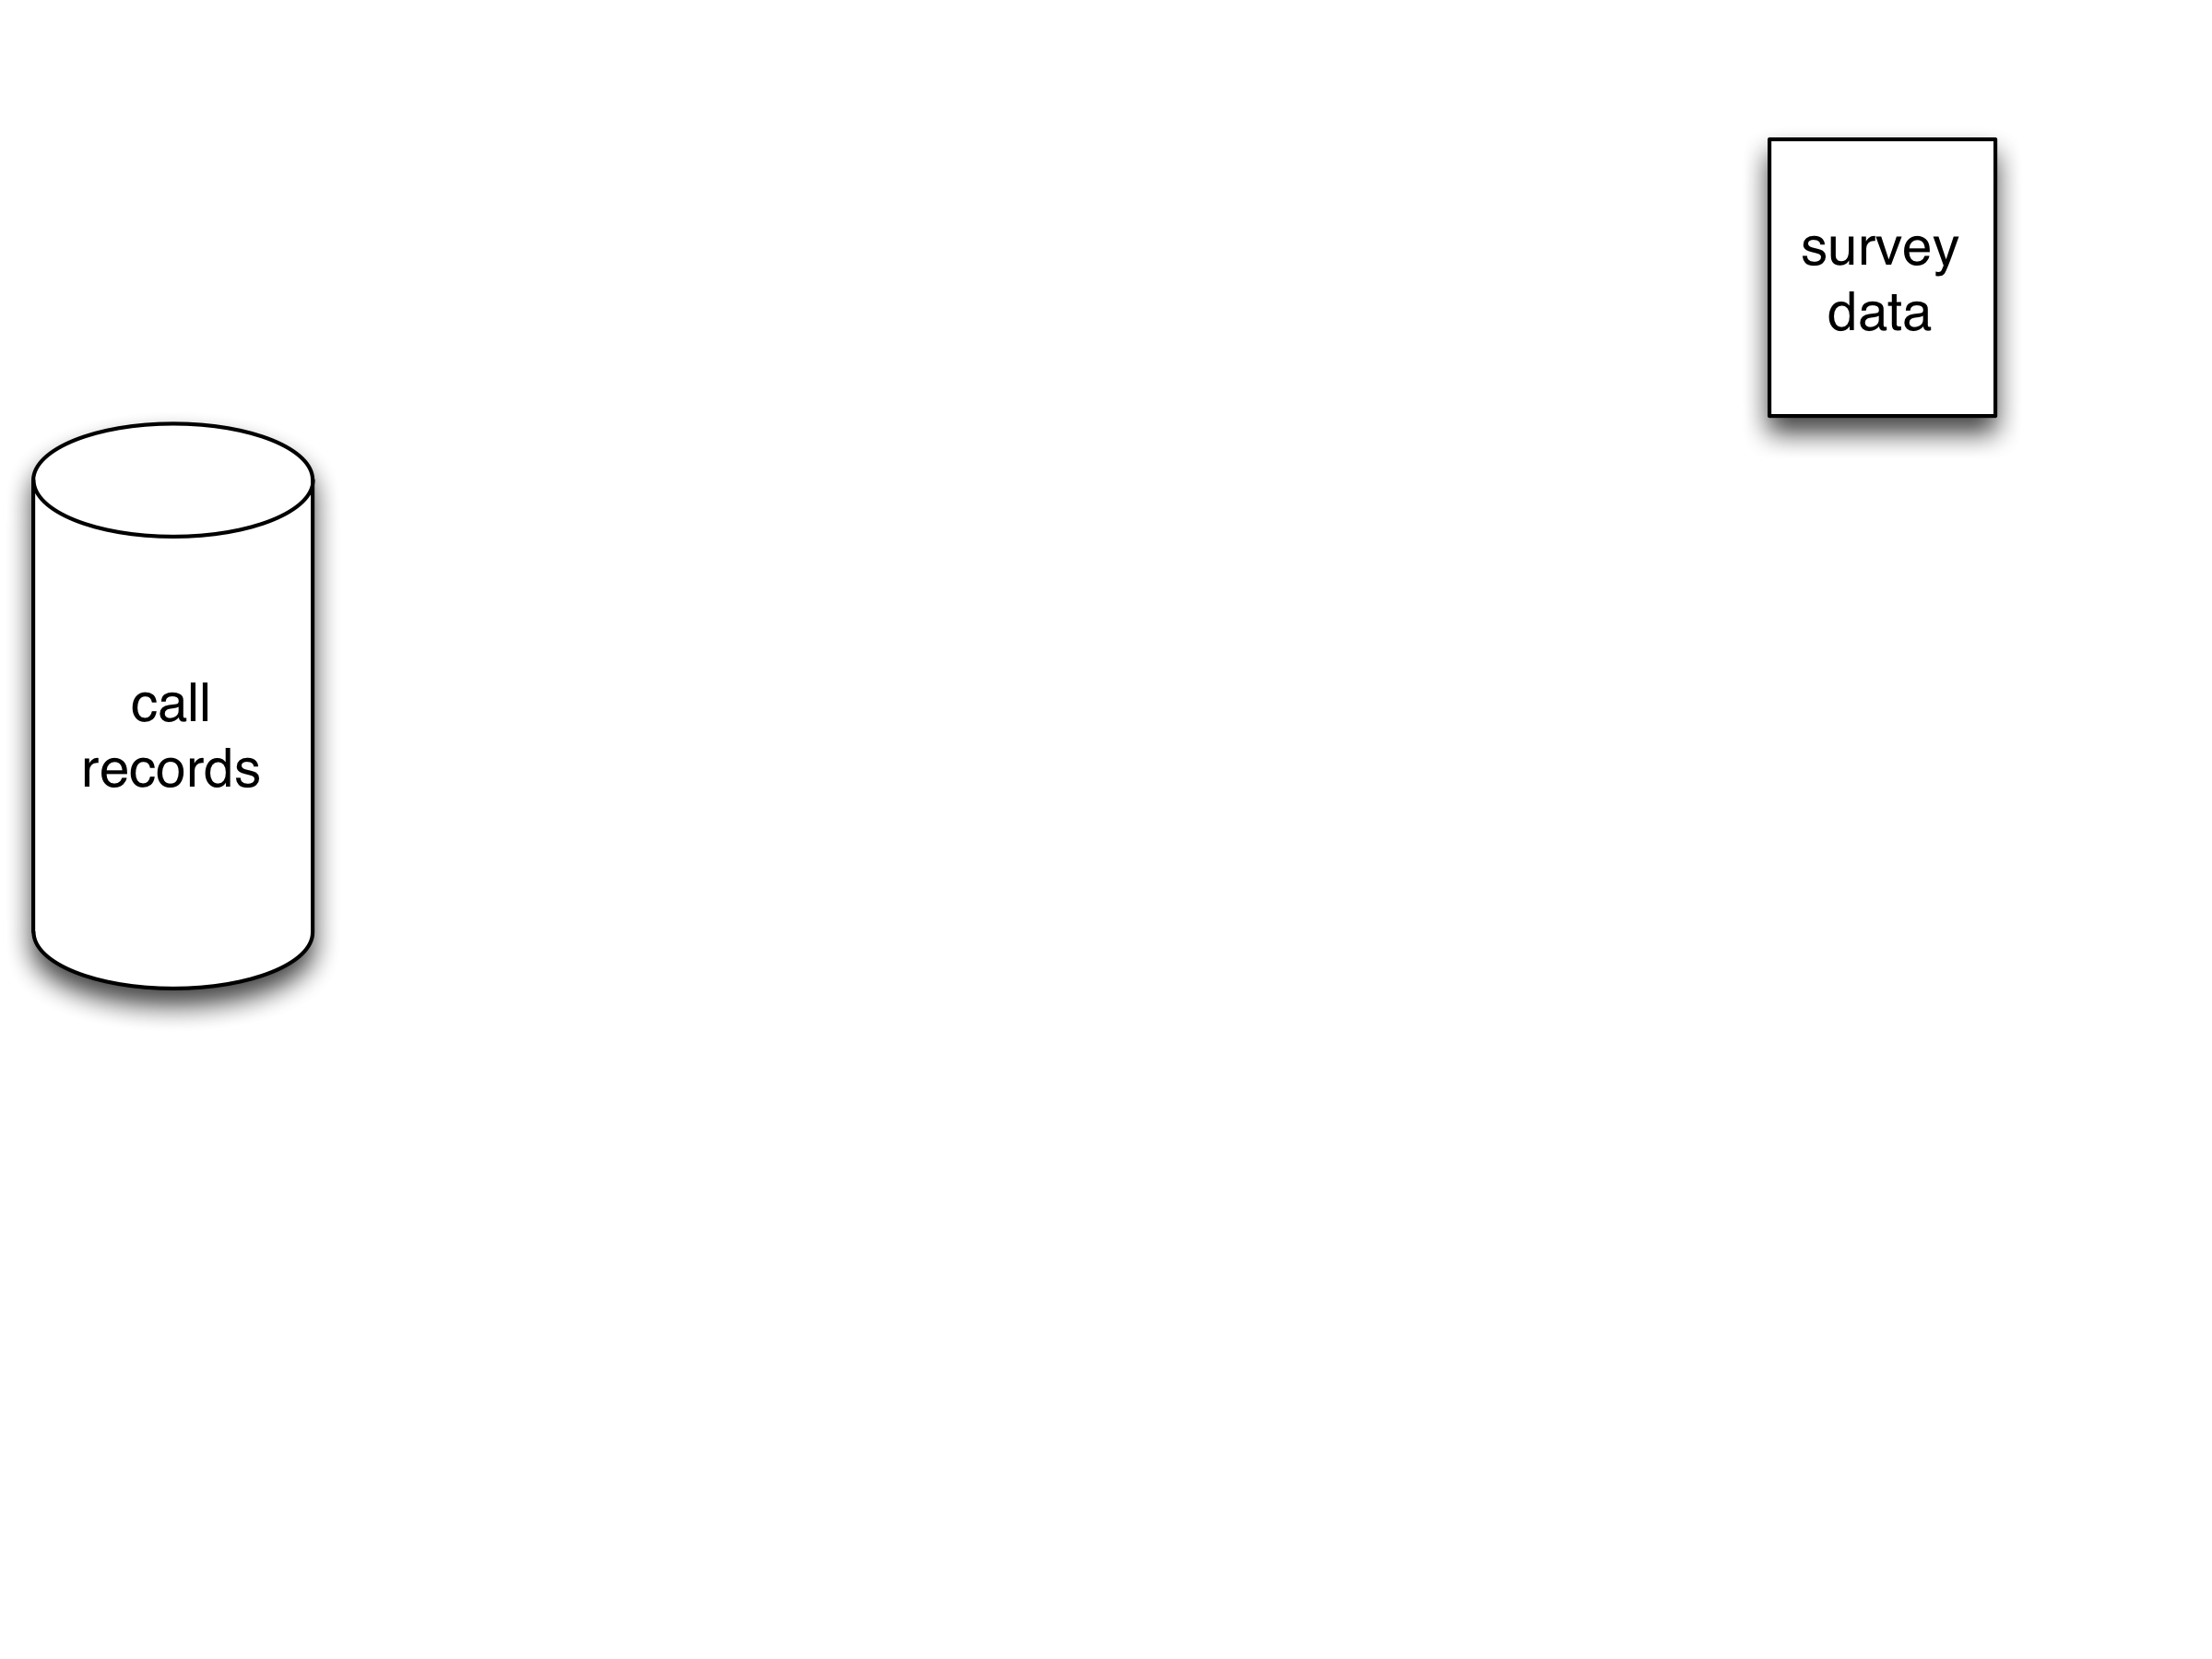
\includegraphics[width=0.9\textwidth]{figures/blumenstock_predicting_2015_schematic_2}}
\only<3>{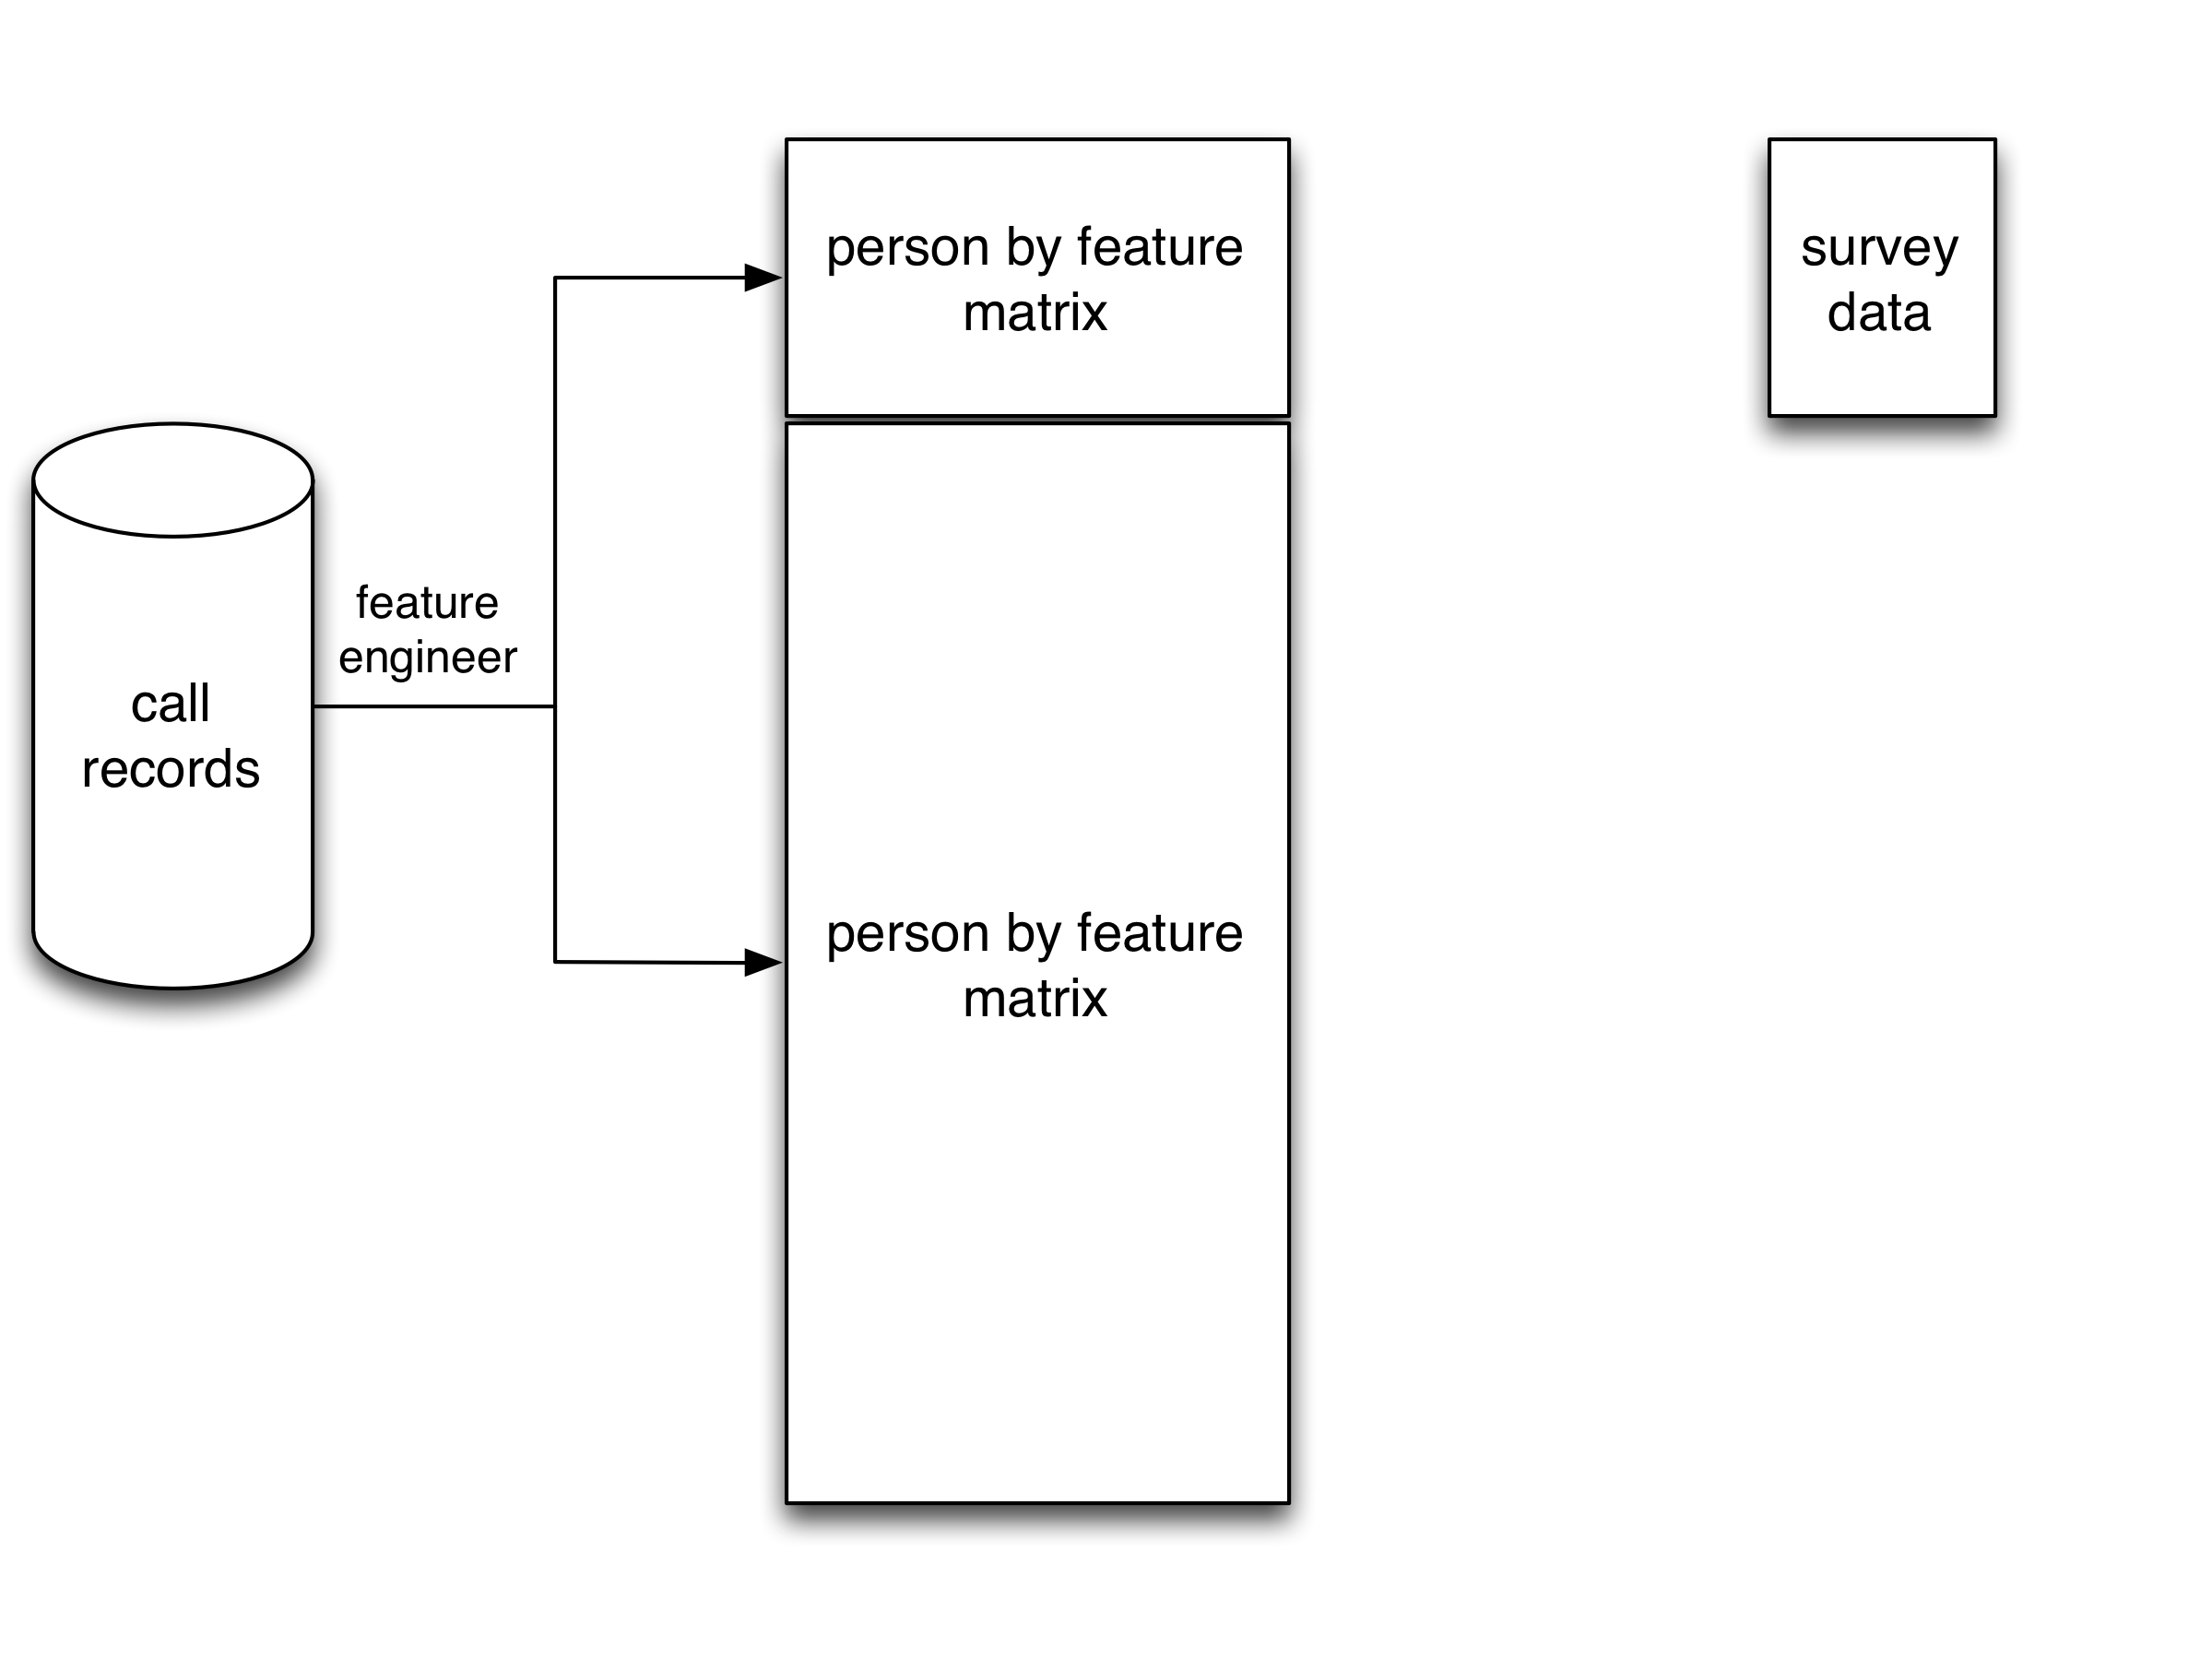
\includegraphics[width=0.9\textwidth]{figures/blumenstock_predicting_2015_schematic_3}}
\only<4>{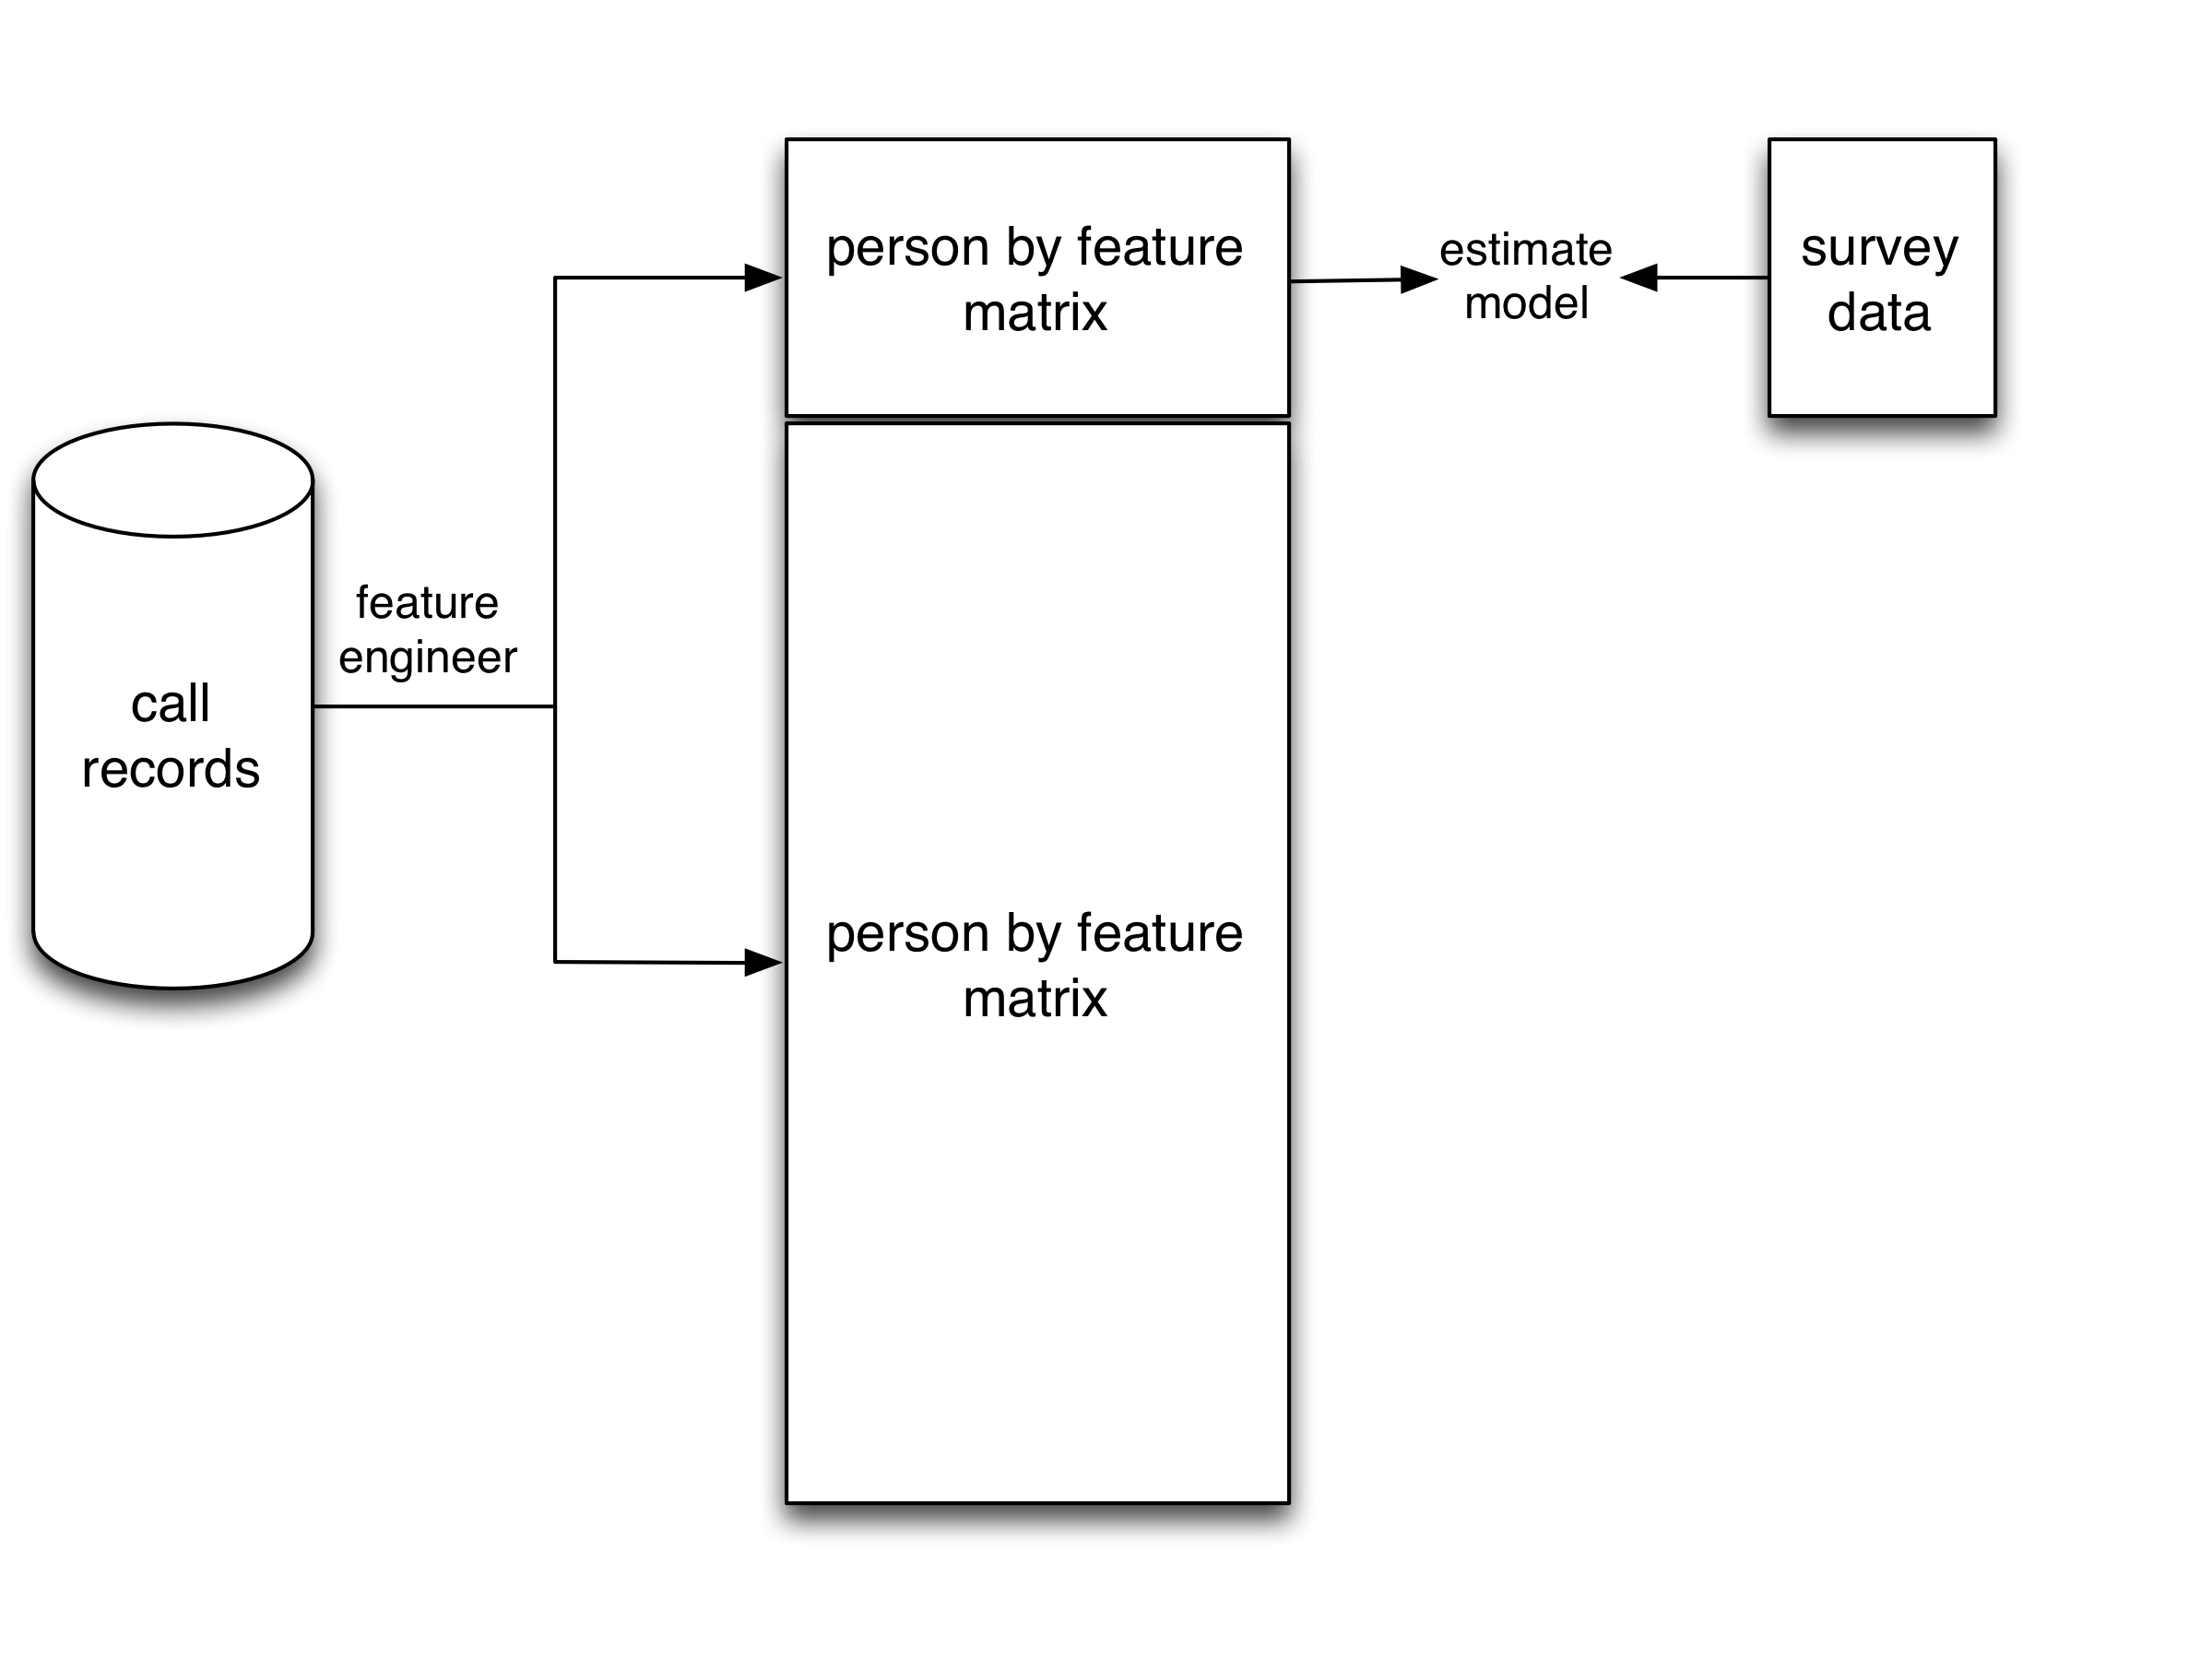
\includegraphics[width=0.9\textwidth]{figures/blumenstock_predicting_2015_schematic_4}}
\only<5>{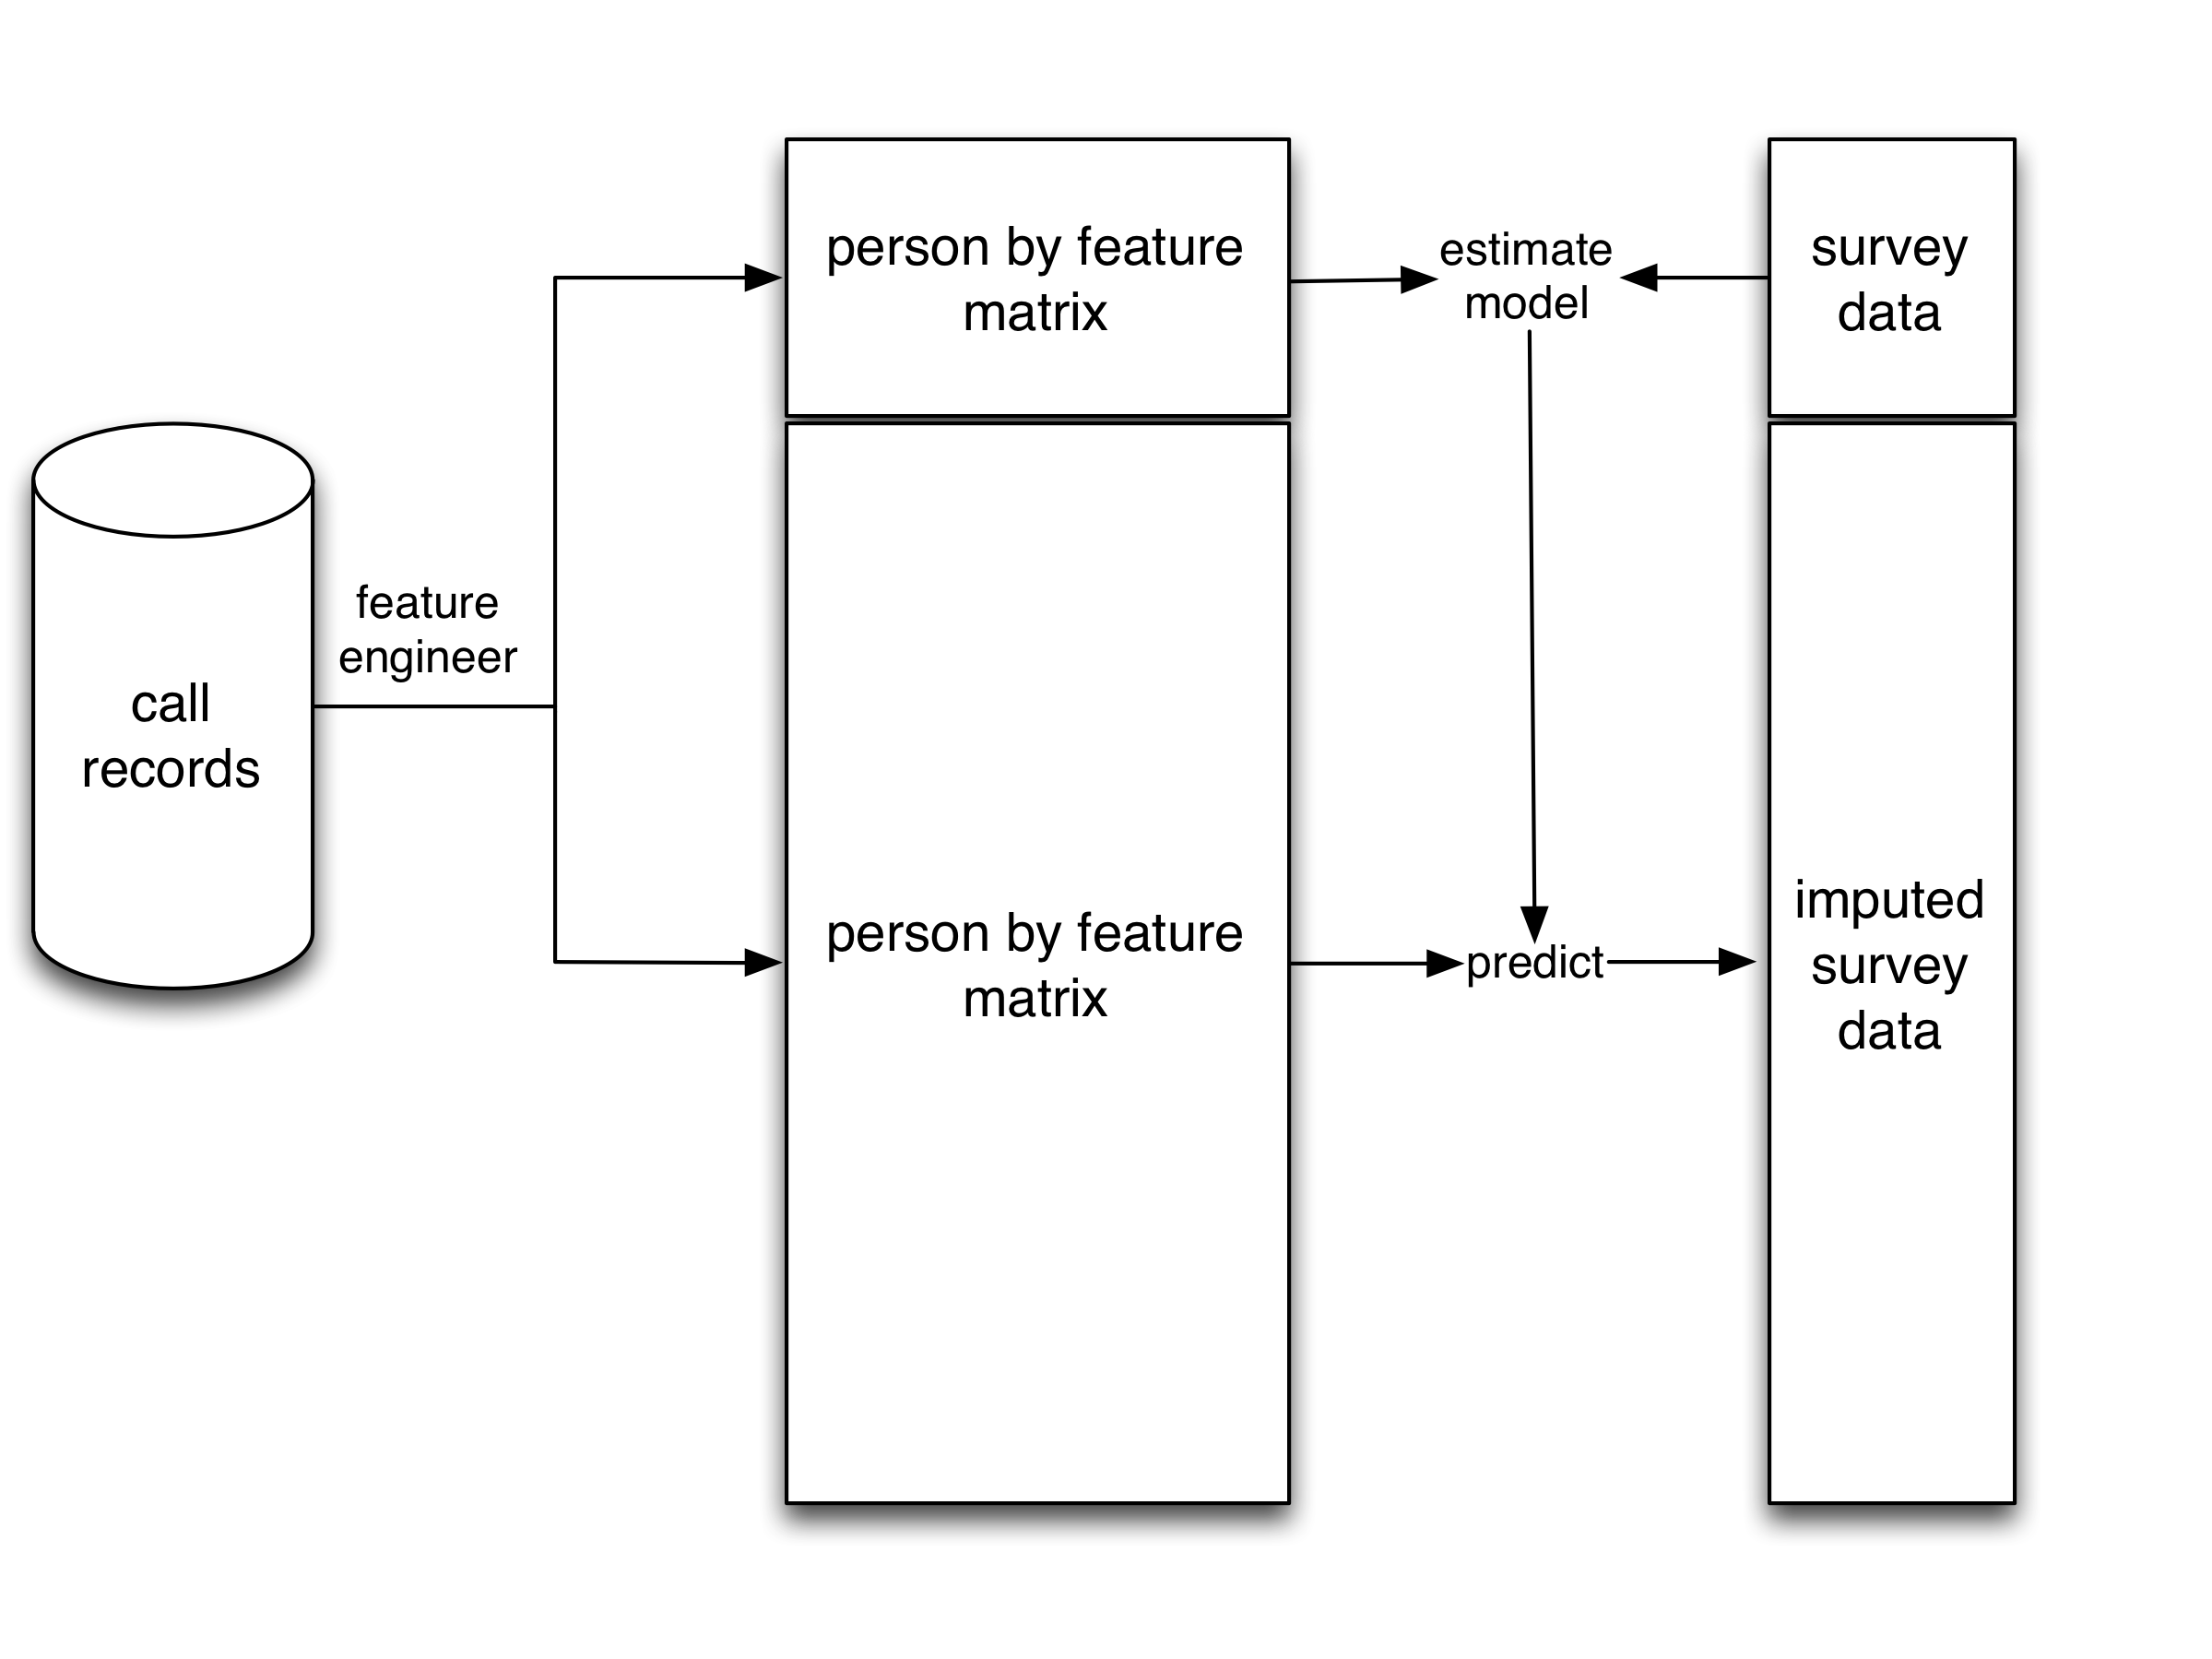
\includegraphics[width=0.9\textwidth]{figures/blumenstock_predicting_2015_schematic_5}}
\only<6>{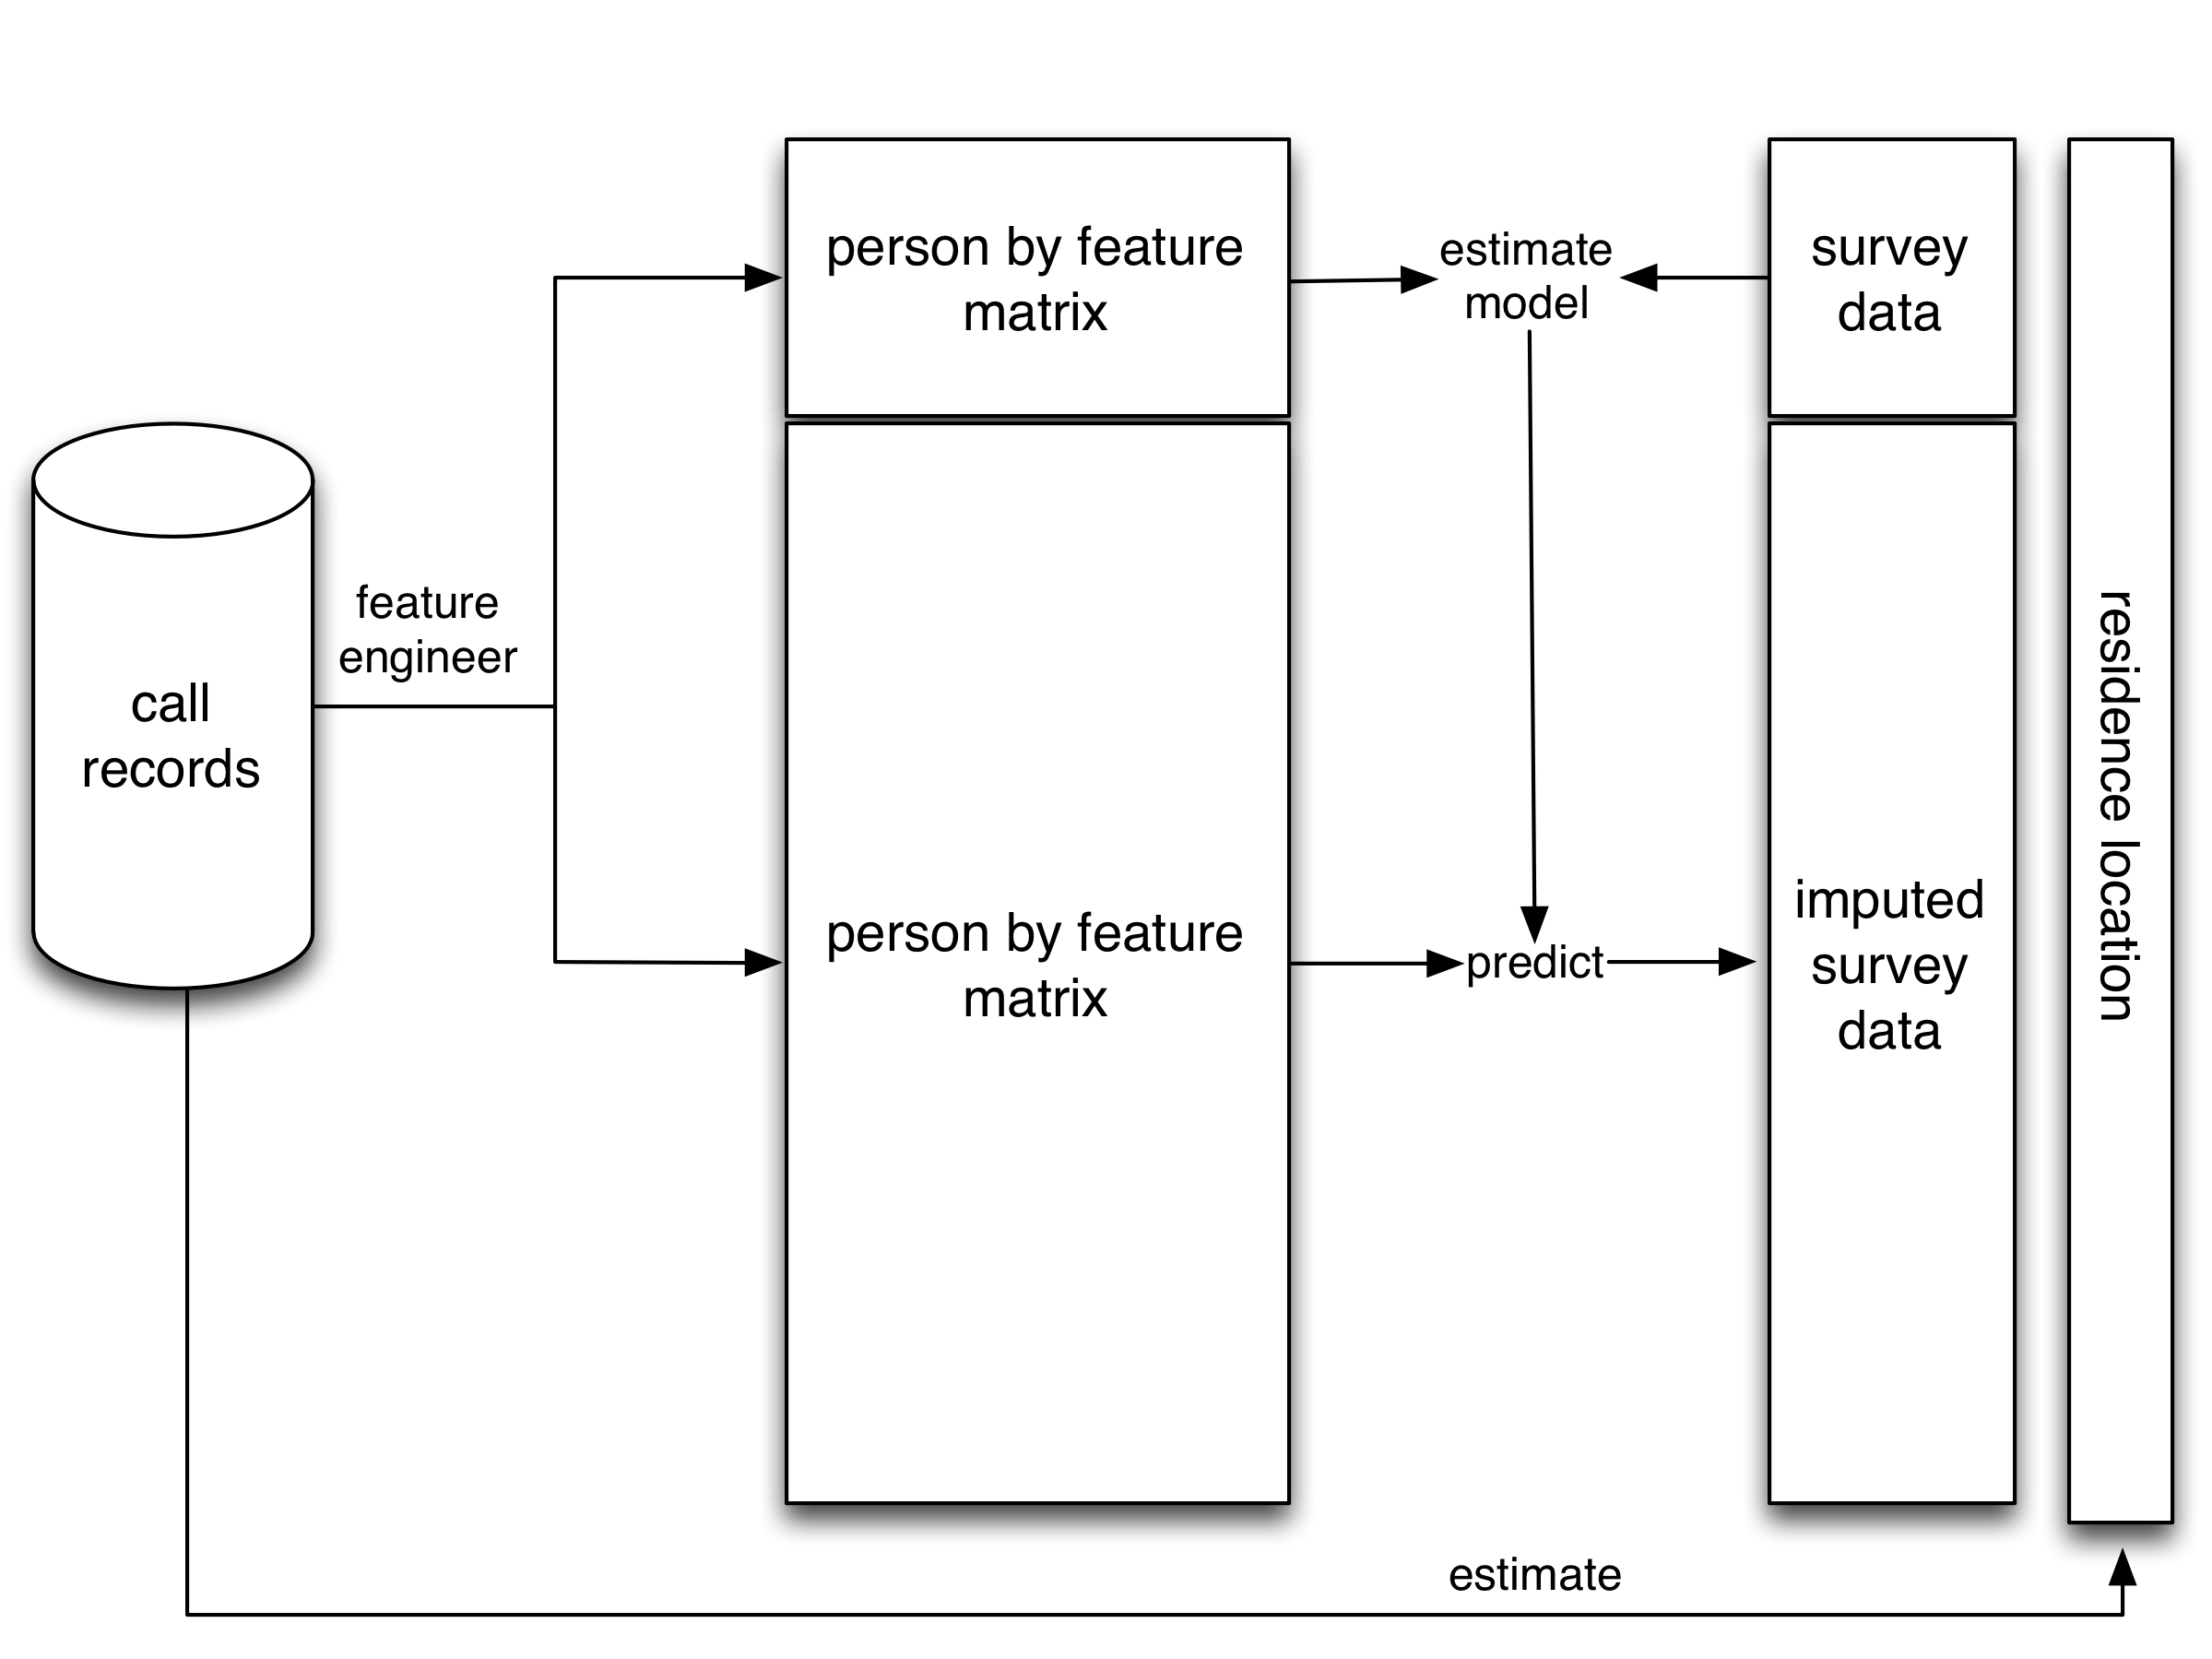
\includegraphics[width=0.9\textwidth]{figures/blumenstock_predicting_2015_schematic_6}}
\end{center}

\end{frame}
%%%%%%%%%%%%%%%%%%%%%%%%%%%
\begin{frame}

\begin{center}
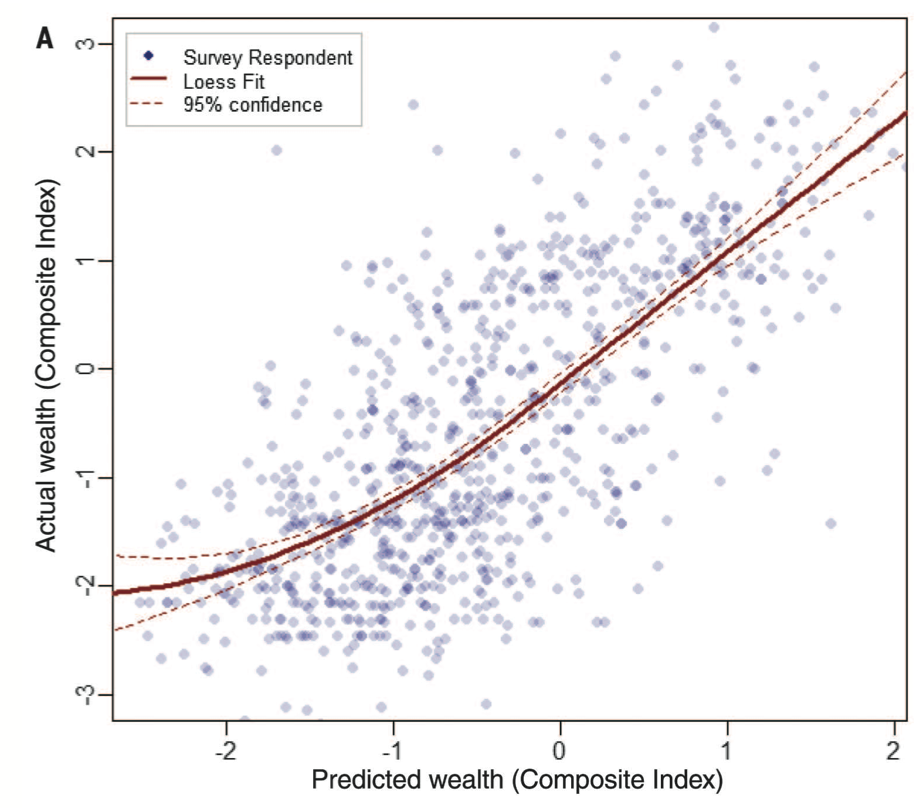
\includegraphics[width=0.8\textwidth]{figures/blumenstock_predicting_2015_fig1a}
\end{center}

\vf
\TINY{\textcolor{blue}{\url{http://dx.doi.org/10.1126/science.aac4420}}}

\end{frame}
%%%%%%%%%%%%%%%%%%%%%%%%%%
\begin{frame}

\begin{center}
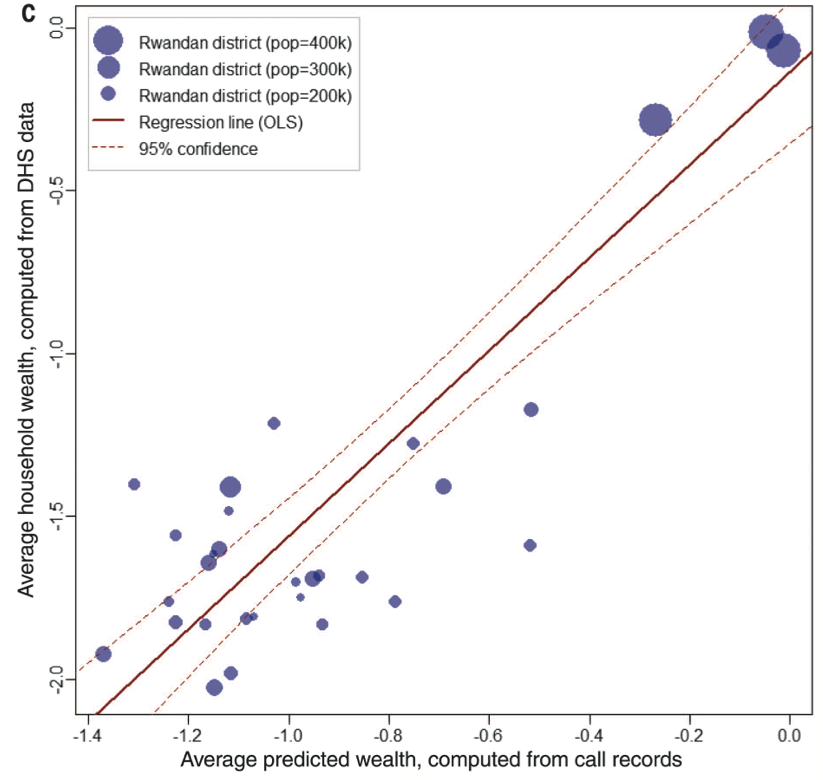
\includegraphics[width=0.65\textwidth]{figures/blumenstock_predicting_2015_fig3c}
\end{center}

\pause

\begin{itemize}
\item 10 times faster
\item 50 times cheaper
\end{itemize}

\vf
\TINY{\textcolor{blue}{\url{http://dx.doi.org/10.1126/science.aac4420}}}
\end{frame}
%%%%%%%%%%%%%%%%%%%%%%%%%%
\begin{frame}

\begin{itemize}
\item \emph{computational} and \emph{social science}
\pause
\item often involves ethical/privacy questions that are now considered complex
\pause
\item combines readymades and customades
\end{itemize}

\end{frame}
%%%%%%%%%%%%%%%%%%%%%%%%%%%
\begin{frame}

\begin{center}
\begin{tabular}{ccc}
\onslide<1-3>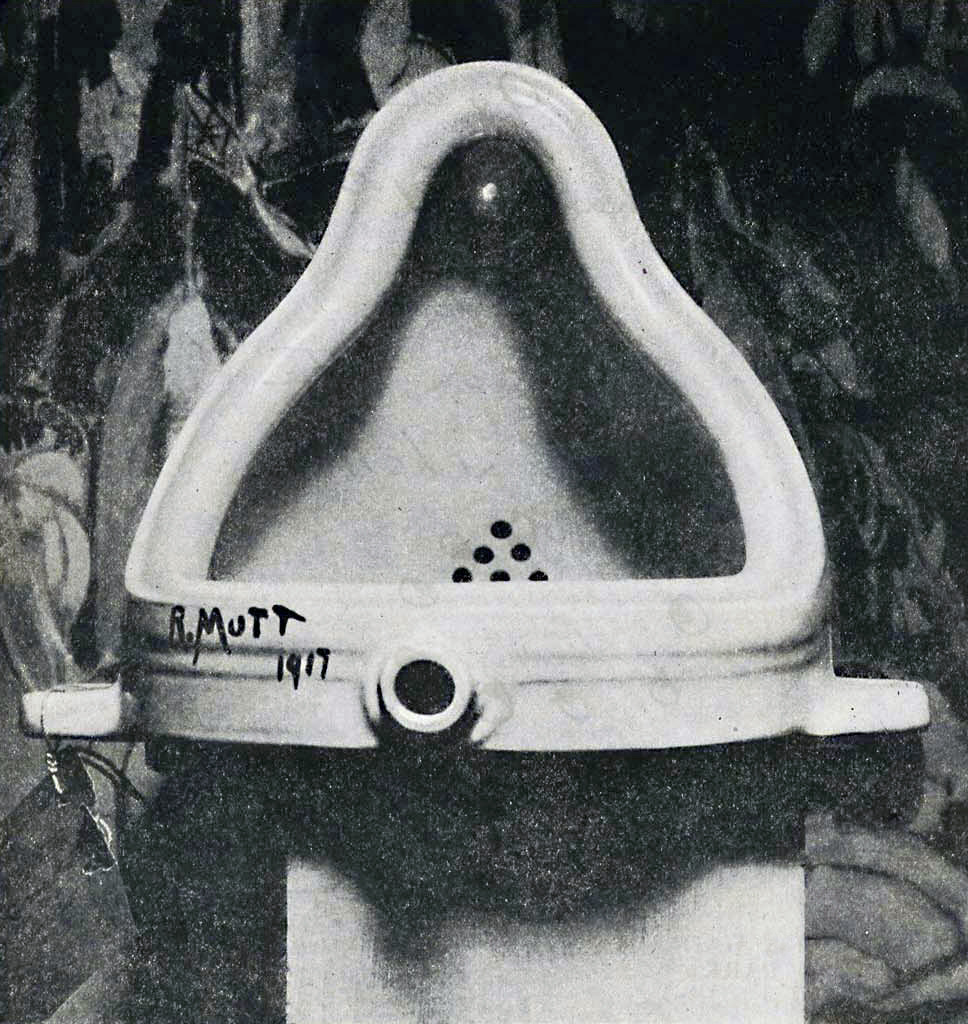
\includegraphics[width=0.30\textwidth]{figures/duchamp_fountain} & \phantom{12345} & \onslide<2-3>{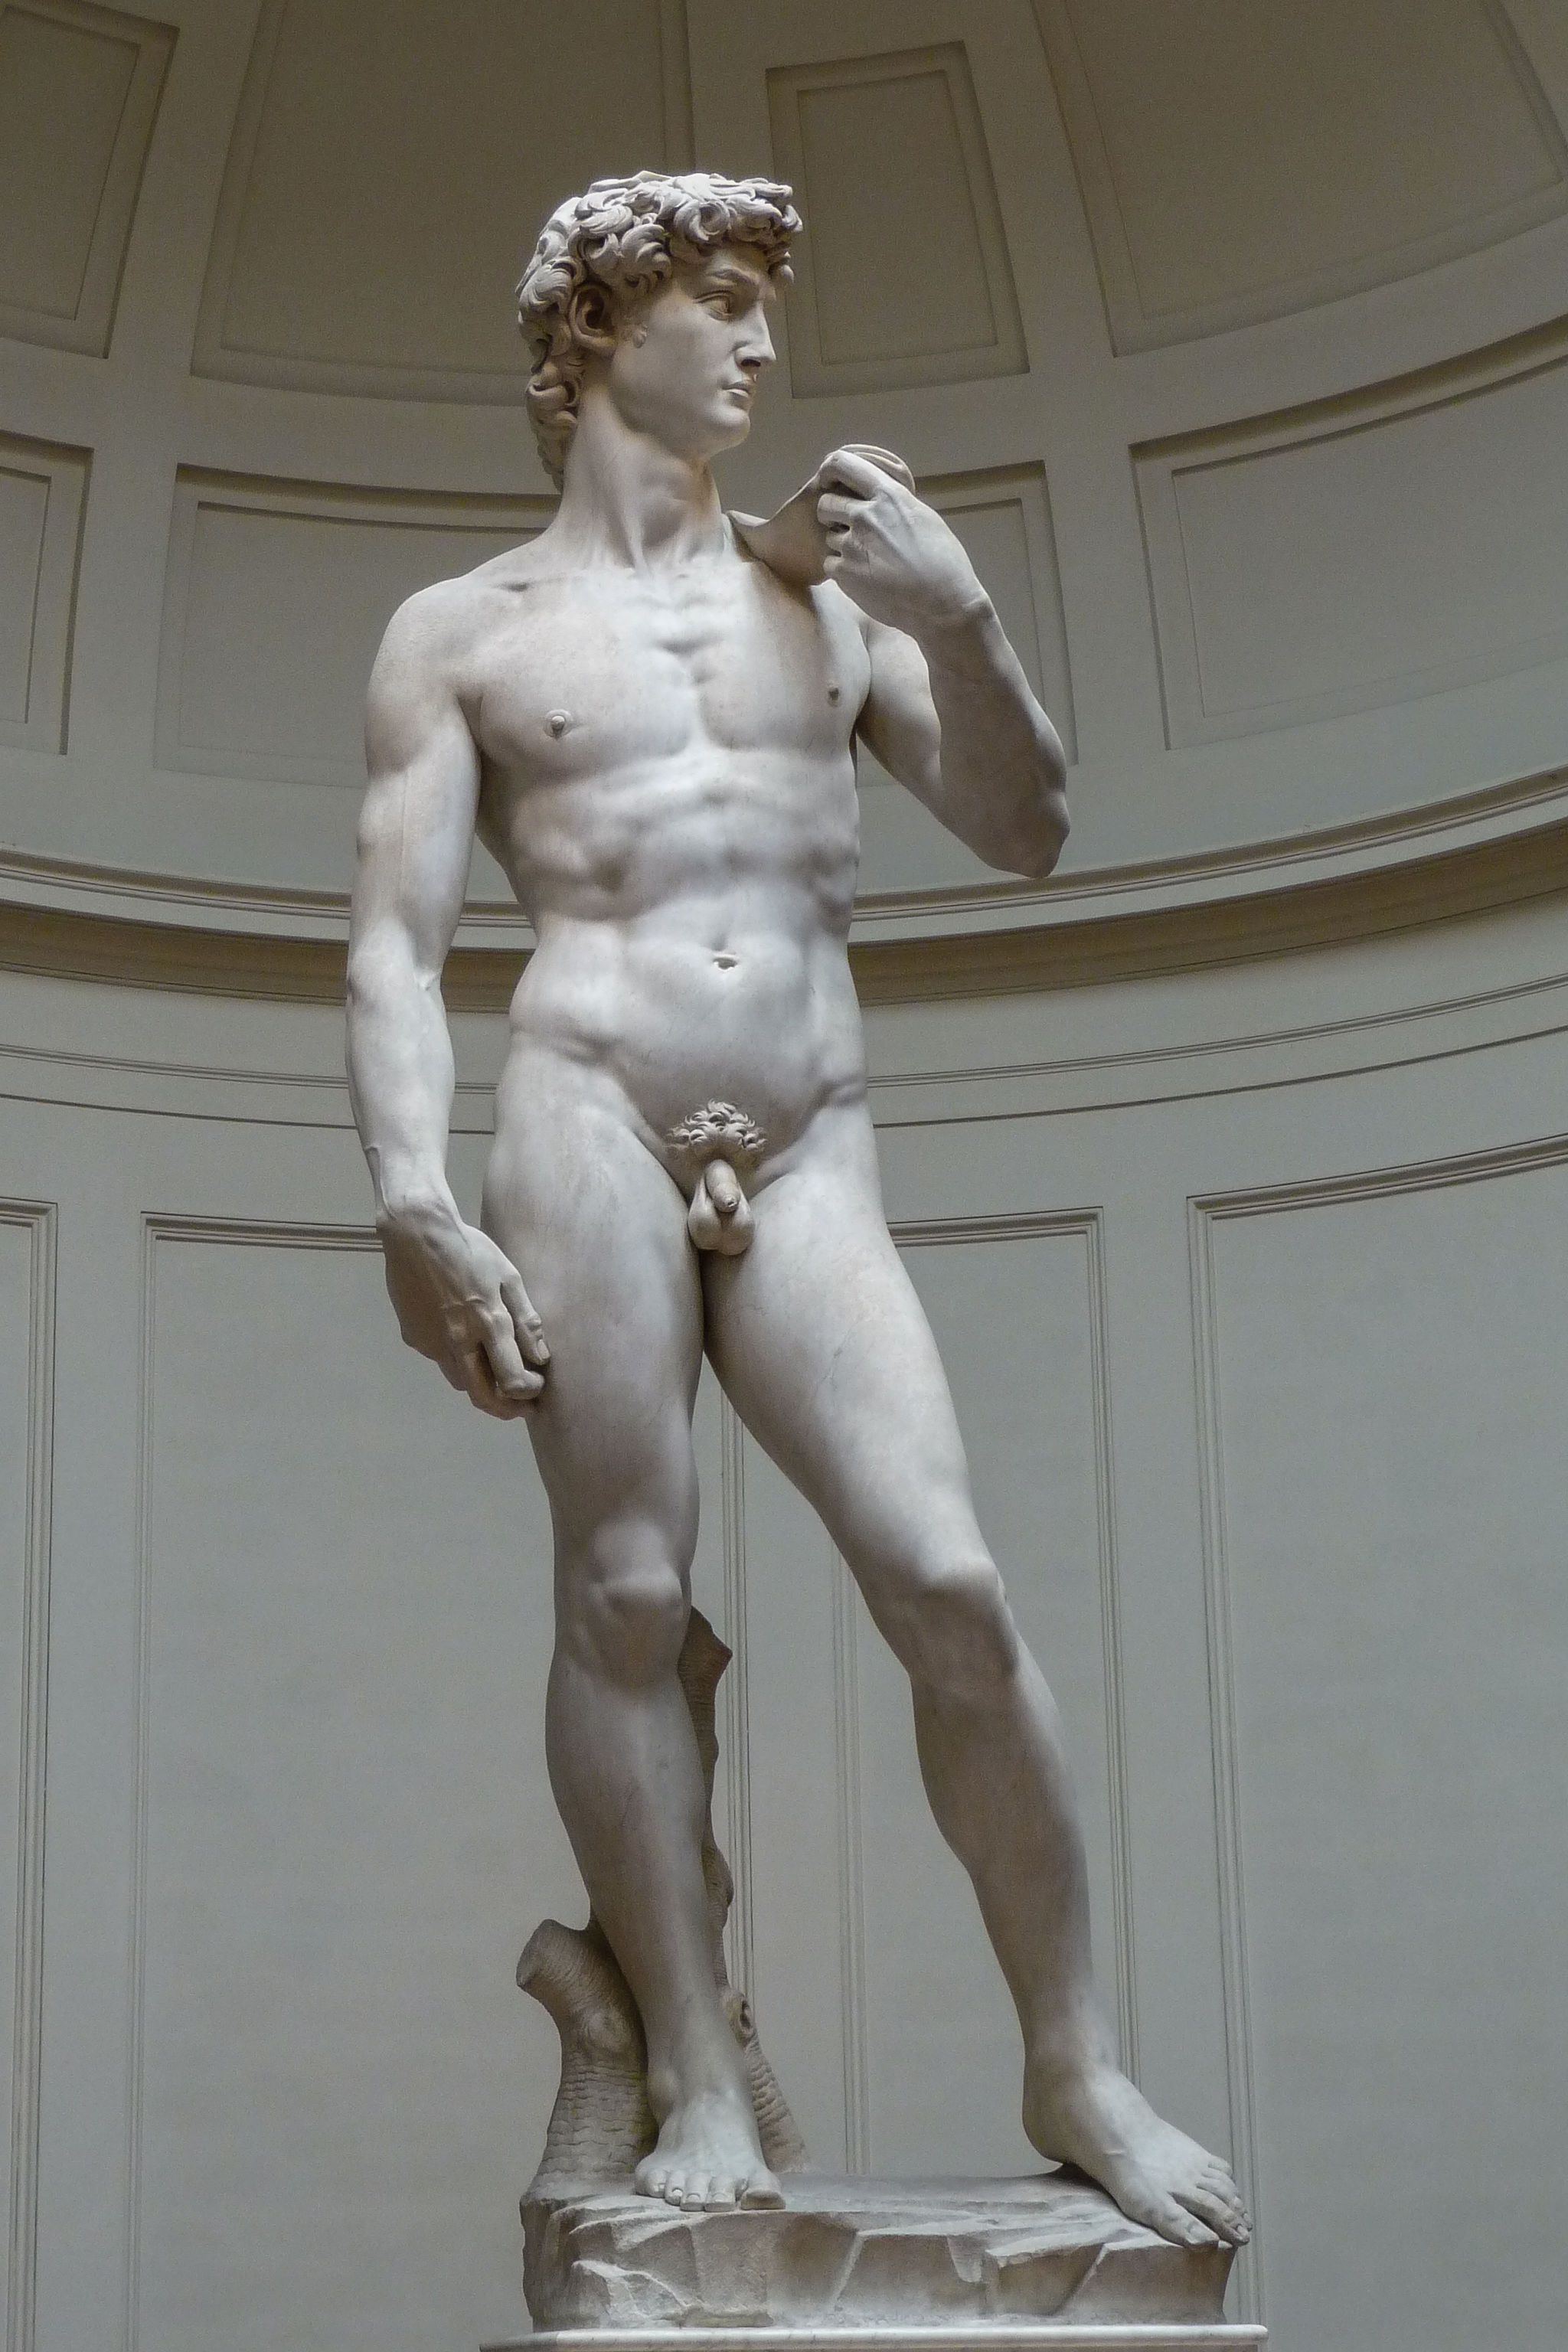
\includegraphics[width=0.30\textwidth]{figures/michelangelo_david}} \\
\onslide<3>{\LARGE{Readymades}} &  & \onslide<3>{\LARGE{Custommades}}
\end{tabular}
\end{center}

\vf
\vspace{0.5in}
\onslide<3>{
\TINY{\url{https://commons.wikimedia.org/wiki/File:Duchamp_Fountaine.jpg}}\\
\TINY{\url{https://commons.wikimedia.org/wiki/File:\%27David\%27_by_Michelangelo_JBU0001.JPG}}}

\end{frame}
%%%%%%%%%%%%%%%%%%%%%%%%%%%
\begin{frame}

\begin{itemize}
\item \emph{computational} and \emph{social science}
\item often involves ethical/privacy questions that are now considered complex
\item combines readymades and custommades
\pause
\item involves five key communities: social science, data science, business people, privacy advocates, policy makers
\end{itemize}

\end{frame}
%%%%%%%%%%%%%%%%%%%%%%%%%%%%
\begin{frame}

\begin{center}
Balance between social science, data science, business people, privacy advocates, and policy markers\\
\end{center}
\vf
\begin{center}
Health Ecosystem vs Horrific Monoculture
\end{center}

\end{frame}
%%%%%%%%%%%%%%%%%%%%%%%%%%%
\begin{frame}

\begin{center}
\LARGE{What is computational social science?}
\end{center}

\begin{itemize}
\item \emph{computational} and \emph{social science}
\item often involves ethical/privacy questions that are now considered complex
\item combines readymades and custommades
\item involves five key communities: social science, data science, business people, privacy advocates, policy makers
\end{itemize}

\end{frame}
%%%%%%%%%%%%%%%%%%%%%%%%%%%
\begin{frame}

\begin{center}
\LARGE{Isn't computational social science a fad?}
\end{center}

\end{frame}
%%%%%%%%%%%%%%%%%%%%%%%%%%%
\begin{frame}

\begin{center}
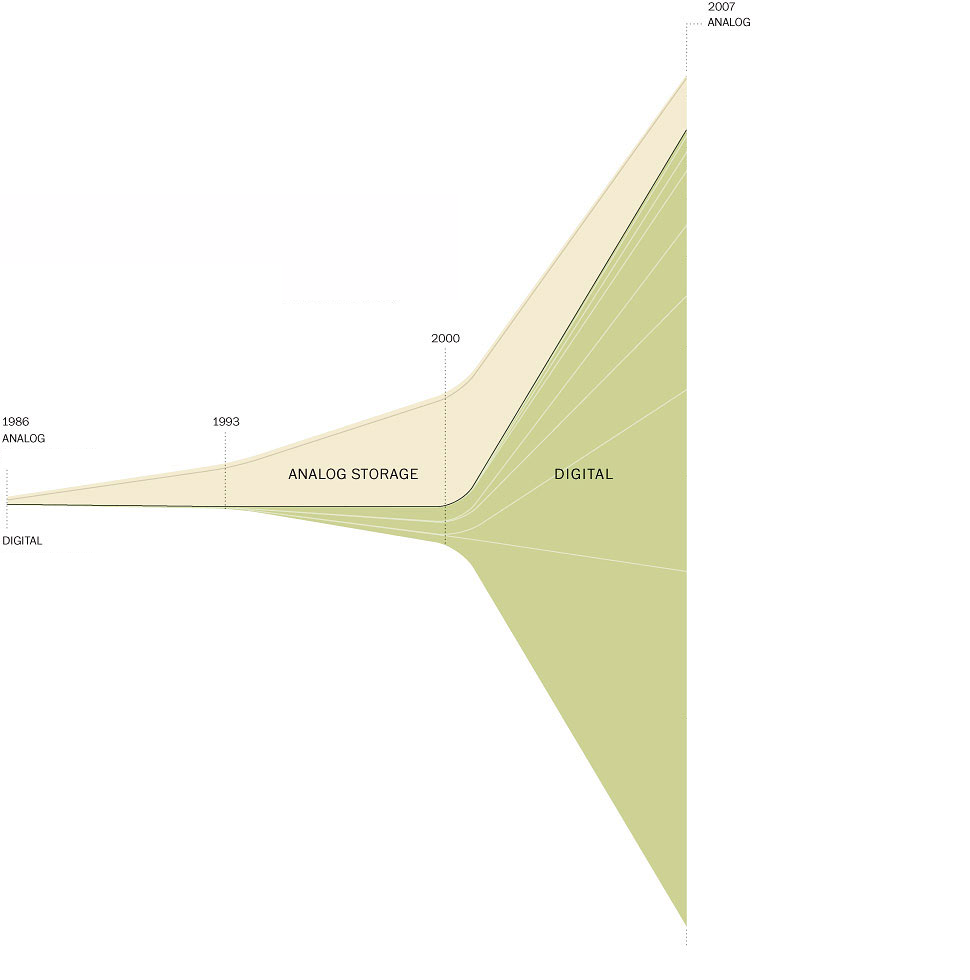
\includegraphics[height=0.9\textheight]{figures/digital_age_clean.png}
\end{center}

\vf
\Tiny{\url{http://www.washingtonpost.com/wp-dyn/content/graphic/2011/02/11/GR2011021100614.html}, based on Hilbert and L\`{o}pez (2011)}

\end{frame}
%%%%%%%%%%%%%%%%%%%%%%%%%%%
\begin{frame}

\begin{center}
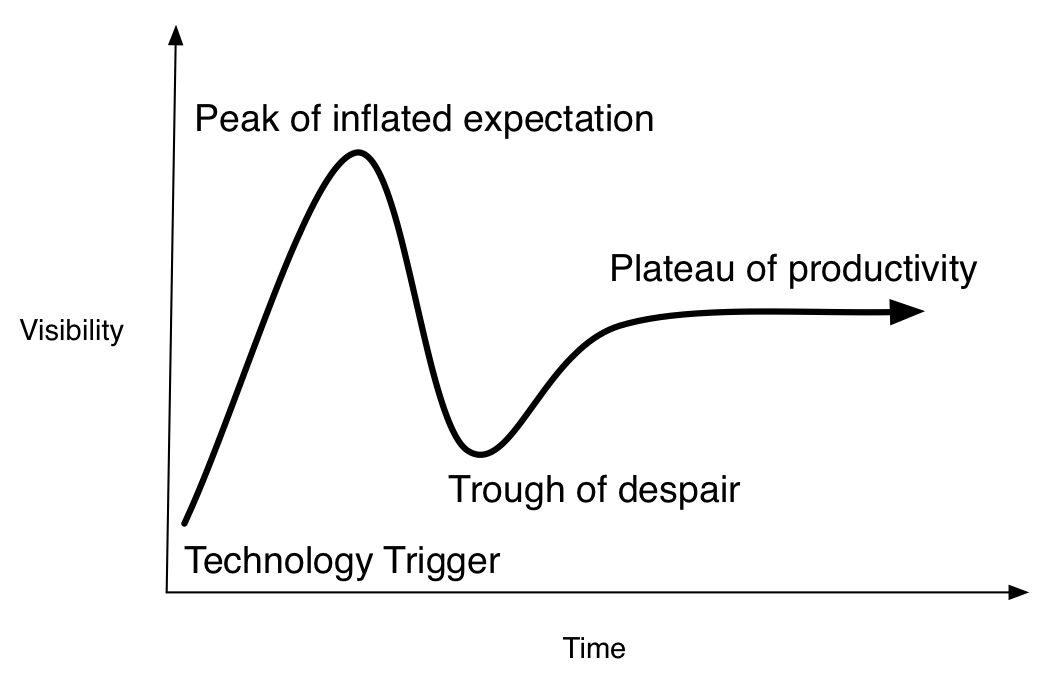
\includegraphics[width=\textwidth]{figures/hype_cycle}
\end{center}

\vf
\Tiny{\url{https://commons.wikimedia.org/wiki/File:Gartner_Hype_Cycle.svg}}

\end{frame}
%%%%%%%%%%%%%%%%%%%%%%%%%%%
\begin{frame}

\begin{center}
\LARGE{Isn't computational social science a fad?}
\end{center}

No

\end{frame}
%%%%%%%%%%%%%%%%%%%%%%%%%%%
\begin{frame}

\begin{center}
\LARGE{How do we create computational social science, individually and as a community?}
\end{center}

\end{frame}
%%%%%%%%%%%%%%%%%%%%%%%%%%%%
\begin{frame}

\begin{center}
\LARGE{Social Scientists $\longleftrightarrow$ Data Scientists}
\end{center}

\end{frame}
%%%%%%%%%%%%%%%%%%%%%%%%%%%
\begin{frame}

\begin{center}
\LARGE{What is data science?}
\end{center}

\end{frame}
%%%%%%%%%%%%%%%%%%%%%%%%%%%
\begin{frame}

\begin{center}
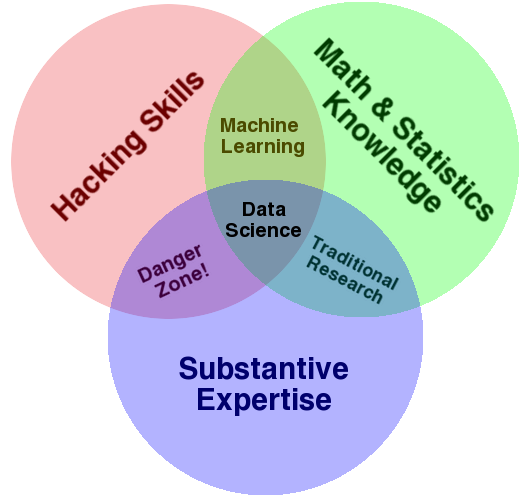
\includegraphics[height=0.9\textheight]{figures/Data_Science_VD.png}
\end{center}

\vf
\Tiny{\textcolor{blue}{\url{http://drewconway.com/zia/2013/3/26/the-data-science-venn-diagram}}}

\end{frame}
%%%%%%%%%%%%%%%%%%%%%%%%%%%%
\begin{frame}

\begin{center}
\LARGE{What is data science?}
\end{center}
Academic data science and industrial data science

\end{frame}
%%%%%%%%%%%%%%%%%%%%%%%%%%%
\begin{frame}

Academic data science (think of Donoho article)\\
\begin{itemize}
\item goes back to Tukey (1962)
\pause
\item learning from data
\pause
\item it includes statistics and much more
\end{itemize}

\end{frame}
%%%%%%%%%%%%%%%%%%%%%%%%%%%
\begin{frame}

Industrial data science (think of Provost and Fawcett)
\begin{itemize}
\item lots of engineering
\pause
\item certain kinds of problems---churn and pop-tarts---that are not as far from social science as they appear
\end{itemize}

\end{frame}
%%%%%%%%%%%%%%%%%%%%%%%%%%%
\begin{frame}

Data science alone is not enough if we want to study social behavior (e.g., Anderson)\\
\pause
Social science alone is not enough if we want to use new data sources

\end{frame}
%%%%%%%%%%%%%%%%%%%%%%%%%%%
\begin{frame}

Wallach (2015) reports overhearing: ``I don't get it.  Why is that research?''\\
\pause
\vf
\begin{center}
\begin{tabular}{cc}
Computer science & Social science\\
\midrule
Study anything & Study social things\\
Methods driven & Question driven\\
Large found data & Small designed data\\
Prediction & Explanation\\
\end{tabular}
\end{center}

\vf
\Tiny{\url{http://videolectures.net/icml2015_wallach_social_science/}}

\end{frame}
%%%%%%%%%%%%%%%%%%%%%%%%%%%
\begin{frame}

Another important difference between social science and data science:
\begin{center}
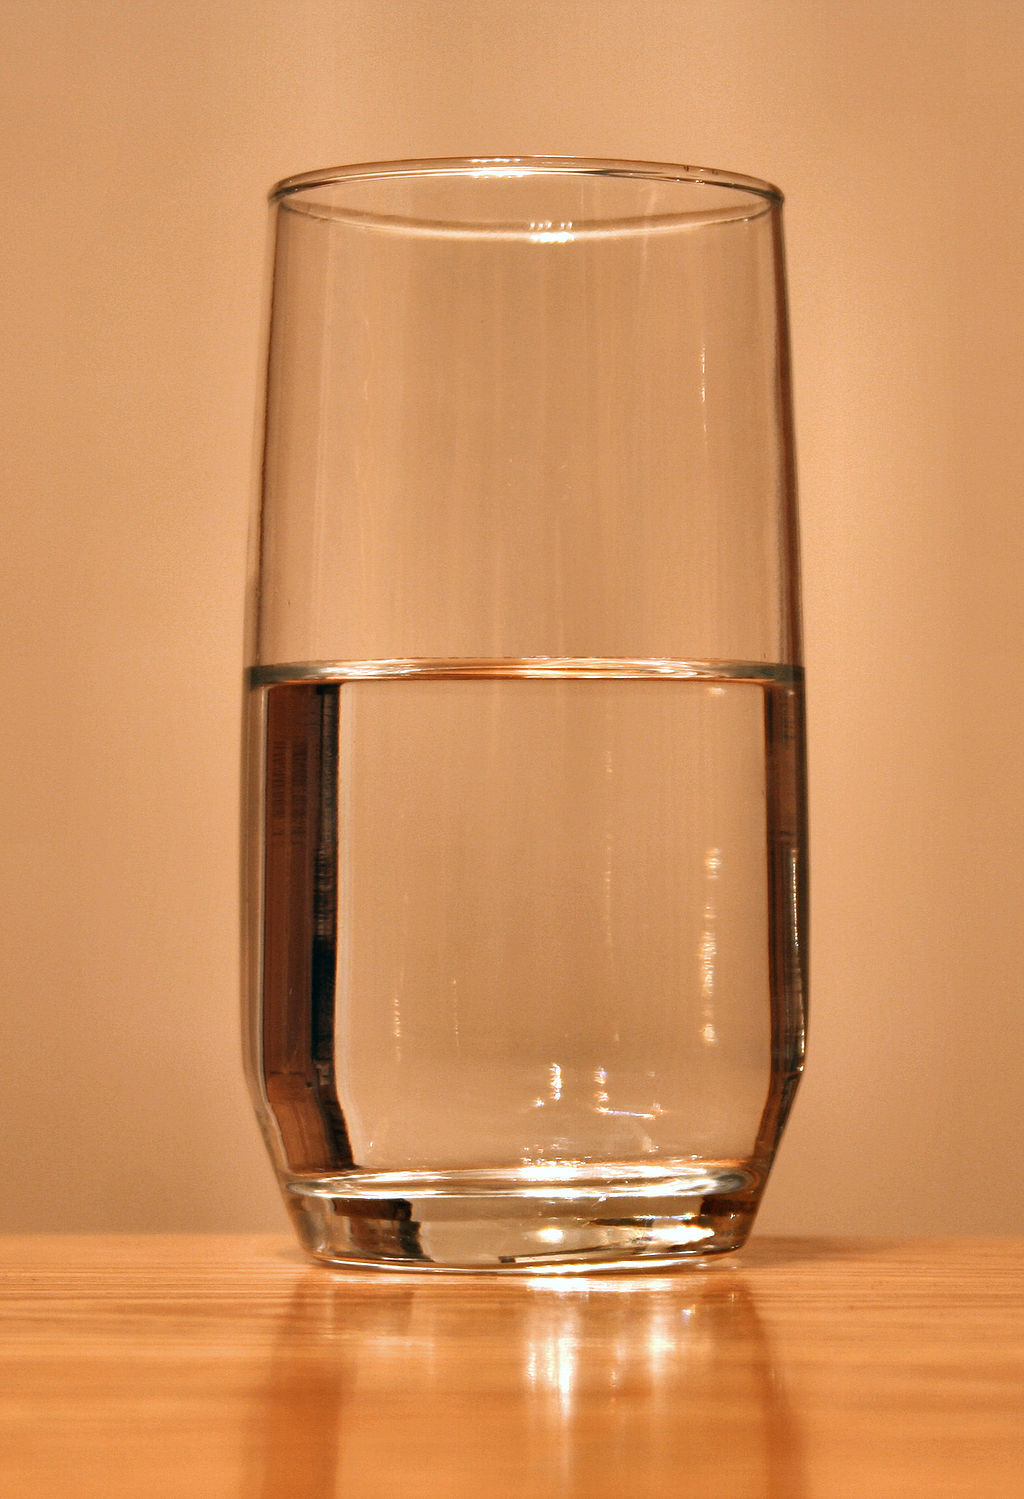
\includegraphics[height=0.7\textheight]{figures/glass-of-water.jpg}
\end{center}

\vf
\vspace{0.5in}
\TINY{\url{https://commons.wikimedia.org/wiki/File:Glass-of-water.jpg}}\\
\end{frame}
%%%%%%%%%%%%%%%%%%%%%%%%%%%
\begin{frame}

\begin{center}
\LARGE{Social Scientists $\longleftrightarrow$ Data Scientists}
\end{center}

\end{frame}
%%%%%%%%%%%%%%%%%%%%%%%%%%%
\begin{frame}

\emph{Computational} social science vs Computational \emph{social science}

\end{frame}
%%%%%%%%%%%%%%%%%%%%%%%%%%%
\begin{frame}

\begin{center}
\Large{Simplicity vs Complexity}
\end{center}

\end{frame}
%%%%%%%%%%%%%%%%%%%%%%%%%%%
\begin{frame}

My goals for this module:
\begin{itemize}
\item SWBAT \emph{describe} computational social science
\item SWBAT \emph{assess} whether computational social science is a fad
\item SWBAT \emph{describe} the intellectual traditions that underly computational social science
\end{itemize}

\end{frame}
%%%%%%%%%%%%%%%%%%%%%%%%%%
%%%%%%%%%%%%%%%%%%%%%%%%%%
%%%%%%%%%%%%%%%%%%%%%%%%%%
%%%%%%%%%%%%%%%%%%%%%%%%%%
%%%%%%%%%%%%%%%%%%%%%%%%%%
%%%%%%%%%%%%%%%%%%%%%%%%%%

\end{document}
